% ESP32 signal chain with the raw-I/Q debug bypass ("ESPARGOS as an SDR").
% Adapted from the KH2026 presentation diagram for the ESPARGOS website.
% Build: pdflatex esp32-sdr-bypass.tex; pdf2svg esp32-sdr-bypass.pdf esp32-sdr-bypass.svg
\documentclass[border=2pt]{standalone}

\renewcommand{\familydefault}{\sfdefault}
\usepackage{helvet}
\usepackage{tikz}
\usetikzlibrary{calc}
\usetikzlibrary{positioning}
\usetikzlibrary{arrows.meta}
\usetikzlibrary{backgrounds}
% Website palette from espargos.scss.
\definecolor{accent}{HTML}{37C964}
\definecolor{surface}{HTML}{293135}
\definecolor{background}{HTML}{11191E}
\definecolor{foreground}{HTML}{DEE2E6}
\definecolor{muted}{HTML}{ADB5BD}
\definecolor{outline}{HTML}{66757D}

\def\ShowBypass{1}

\begin{document}
% Shared ESP32 radio block diagram, used by both Outlook figures:
%   img/esp32-hw-modem.tex   - plain hardware-modem signal chain
%   img/esp32-sdr-bypass.tex - same drawing with \ShowBypass defined, which
%                              adds the raw-I/Q debug bypass in green
% The bounding box is identical in both variants, so the bypass appears as a
% pure overlay when switching between the two slides.
\newcommand{\blocklabel}[2]{%
	{\footnotesize\bfseries\color{accent}#1}\\[-1pt]{\tiny\color{muted}#2}}
\newcommand{\blocklabeldark}[2]{%
	{\footnotesize\bfseries\color{white}#1}\\[-1pt]{\tiny\color{foreground}#2}}
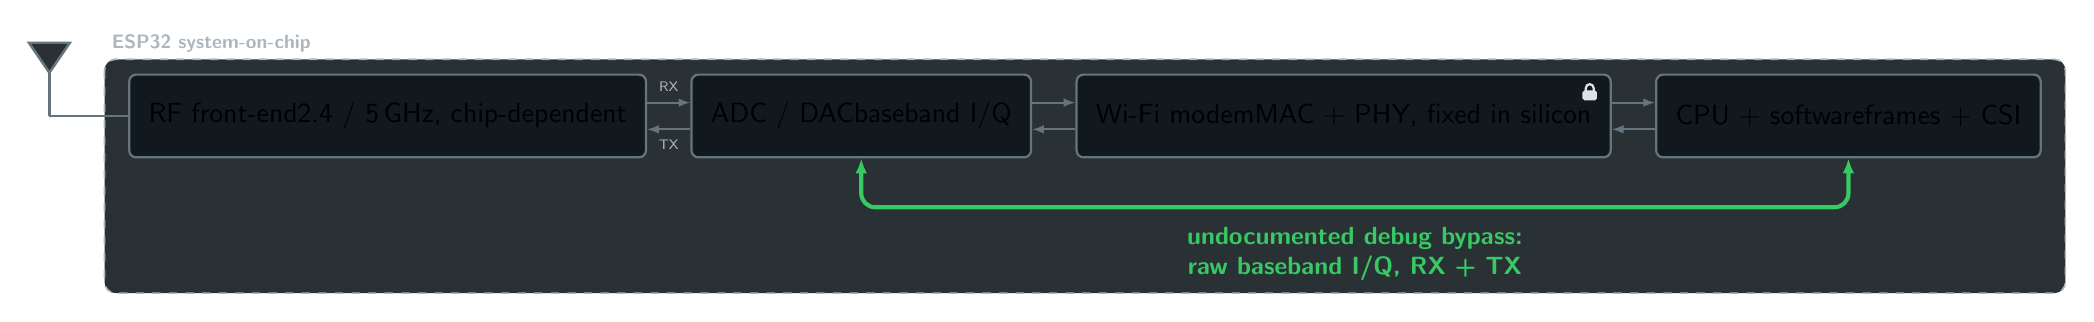
\begin{tikzpicture}[
	block/.style={draw=outline, line width=0.8pt, rounded corners=2.5pt,
		fill=background, minimum height=1.05cm, align=center, inner xsep=7pt},
	sig/.style={-{Latex[length=1.5mm, width=1.1mm]}, line width=0.7pt, outline},
]
	% signal chain
	\node[block] (rf) {\blocklabel{RF front-end}{2.4 / 5\,GHz, chip-dependent}};
	\node[block, right=0.55cm of rf] (adc) {\blocklabel{ADC / DAC}{baseband I/Q}};
	\node[block, right=0.55cm of adc, fill=background] (modem)
		{\blocklabeldark{Wi-Fi modem}{MAC + PHY, fixed in silicon}};
	\node[block, right=0.55cm of modem] (cpu) {\blocklabel{CPU + software}{frames + CSI}};

	% ESP32 package outline, grey-ish like the actual SoC package
	\begin{scope}[on background layer]
		\draw[draw=muted, dashed, line width=0.6pt, rounded corners=4pt,
			fill=surface] ($(rf.west)+(-0.3,0.72)$) rectangle ($(cpu.east)+(0.3,-2.25)$);
	\end{scope}
	\node[anchor=south west, inner sep=2.5pt] at ($(rf.west)+(-0.3,0.72)$)
		{\scriptsize\bfseries\color{muted}ESP32 system-on-chip};

	% antenna
	\coordinate (ant) at ($(rf.west)+(-1.0,0)$);
	\draw[outline, line width=0.8pt] (ant) -- (rf.west);
	\draw[outline, line width=0.9pt] (ant) -- ++(0,0.55);
	\draw[outline, line width=0.9pt, fill=surface]
		($(ant)+(0,0.55)$) -- ++(-0.26,0.38) -- ++(0.52,0) -- cycle;

	% RX (left to right) and TX (right to left) between the chain blocks
	\foreach \a/\b in {rf/adc, adc/modem, modem/cpu} {
		\draw[sig] ($(\a.east)+(0,0.17)$) -- ($(\b.west)+(0,0.17)$);
		\draw[sig] ($(\b.west)+(0,-0.17)$) -- ($(\a.east)+(0,-0.17)$);
	}
	\node at ($(rf.east)!0.5!(adc.west)+(0,0.37)$) {\tiny\color{muted}RX};
	\node at ($(rf.east)!0.5!(adc.west)+(0,-0.37)$) {\tiny\color{muted}TX};

	% padlock on the fixed-function modem
	\coordinate (lock) at ($(modem.north east)+(-0.28,-0.26)$);
	\draw[foreground, line width=0.8pt]
		($(lock)+(-0.05,0.04)$) -- ++(0,0.035) arc[start angle=180, end angle=0, radius=0.05] -- ++(0,-0.035);
	\draw[foreground, fill=foreground, rounded corners=0.6pt]
		($(lock)+(-0.085,-0.075)$) rectangle ($(lock)+(0.085,0.04)$);

	\ifdefined\ShowBypass
		% undocumented debug bypass: raw I/Q straight between ADC/DAC and CPU
		\draw[{Latex[length=1.9mm, width=1.5mm]}-{Latex[length=1.9mm, width=1.5mm]},
			line width=1.5pt, accent, rounded corners=5pt]
			(adc.south) -- ++(0,-0.62) -- ($(cpu.south)+(0,-0.62)$) -- (cpu.south);
		\node[anchor=north, align=center, font=\small\bfseries, text=accent]
			at ($(adc.south)!0.5!(cpu.south)+(0,-0.75)$)
			{undocumented debug bypass:\\raw baseband I/Q, RX + TX};
	\fi
\end{tikzpicture}

\end{document}
